%\addcontentsline{toc}{section}{ВВЕДЕНИЕ}
\section*{Общая характеристика работы}

Большое количество современных систем являются беспроводными. Простота развертывания, мобильность, относительно низкая
стоимость - вот основные преимущества беспроводных систем. Количество мобильных устройств (телефоны, планшетные компьютеры
и т.д.) с каждым годом стремительно растет, только мобильных телефонов в 2011 году было 5.6 миллиарда и покрывало 79.86\%
\cite{wiki_mobilenum} населения земли. Технологии беспроводной связи глубоко проникли во все сферы жизни общества:
обеспечение безопасности с помощью RFID датчиков, предоставление доступа в интернет по техноолгиям 3G, WiFi, 
сотовая связь по различным технологиям (GSM, CDMA, DAMPS). Некоторые из этих систем строятся на основе методики
расширения спектра, которая отвечает современным требованиям по мощности сигнала, а так же по безопасности передаваемых
данных. В основе таких систем лежат шумоподобные (широкополосные) сигналы - ШПС. Вместе с тем растут требования к таким
системам. Применение ШПС ставит ряд специфических задач по обработке информации, обусловленных особенностями ШПС.
Свойства характерные для ШПС, выгодно отличают данный класс систем от класса узкополосных систем, но с другой стороны
оборачивается усложнением методов обработки ШПС.

Изначально методы расширенного спектра применялись при разработке военных систем управления и связи \cite{sklyar} (Глава 12.1).
К концу второй мировой войны расширение спектра применялось в радиолокации для борьбы с преднамеренными помехами, а
в последствии развитие данной технологии объяснялось желанием создать помехоустойчивые системы связи.
В конце 40-х-начале 50-х годов прошлого века Мортимер Рогофф, сотрудник Международной Телефонной и Телеграфной Корпорации (США) (ITT),
провёл эксперимент по передаче информации при помощи псевдошумового сигнала \cite{sklyar} (Глава 12.1.4.2).
Результаты его исследований продемонстрировали возможность построения системы передачи информации с шумоподобными сигналами.
Первые разработки таких систем относились к военным отраслям. Данный факт объясняется рядом особенностей, которыми обладают
сигналы с расширенным спектром, в числе которых — сложность перехвата заложенной в них информации,
высокая помехоустойчивость, а также трудность обнаружения факта работы передатчика. В процессе исследований расширенному спектру
нашлось и другое применение - снижение плотности энергии, высокоточная локация, использовние при множественном доступе
\cite{sklyar} (Глава 12.1)

\underline{Цель работы}

Целью данной работы являлись разработка и исследование нового метода оценки параметров сигнала с расширенным спектром с использованием
итерационной оценки атвокорреляционной функции (АКФ) и авторегрессионной (АР) модели.

\underline{Научная новизна работы}
\begin{enumerate}
      \item {Предложен новый способ детектирования сигнала с расширенным спектром;}
      \item {Предложен алгоритм оптимизации итерационного вычисления АКФ;}
      \item {Подход, предложенный в работе, позволяет произвести точную оценку на ограниченном отрезке сигнала, без накопления;}
      \item {Полученные оценки параметров сигнала являются гораздо более точными в сравнении с классическим алгоритмом
      		параллельного коррелятора.}
\end{enumerate}

\underline{Научная и практическая значимость работы}
\begin{enumerate}
      \item {;}
\end{enumerate}

\underline{Основные научные положения, выносимые на защиту}

\underline{Достоверность научных положений, результатов и выводов}

\underline{Апробация работы}

\underline{Публикации}

\underline{Личный вклад автора}

\underline{Объём и структура диссертации}

\section*{СОДЕРЖАНИЕ РАБОТЫ}

% Include text from phd
\input{lpc}

Точность АР метода напрямую зависит от точности оценки АКФ гармонического сигнала. Основным способом повышения точности оценки АКФ является увеличение размера выборки,
что в случае модулированного сигнала может быть затруднительным.В данной работе предлагается использовать алгоритм увеличения ОСШ мектодом последовательного вычисления
АКФ \cite{ostanin_akf}. Для снижения вычислительных затрат указанный алгоритм предлагается реализовывать с использованием процедуры БПФ. 
Введем следующие обозначения: ${x}$ – вектор входного сигнала после снятия ПСП, ${F}$ – матрица прямого преобразования Фурье, ${F^{-1}}$- матрица обратного преобразования Фурье.
Оценку АКФ на первом шаге можно получить следующим образом:

\begin{center}
\begin{equation}
	\label{eq:akf_1}
	\hat{r_1} = F^{-1}\left[ Fx \cdot (Fx)^* \right] = F^{-1} \left[ \left| Fx \right| ^2 \right]
\end{equation}
\end{center}

Здесь знак ${(\cdot)}$  означает поэлементное перемножение векторов, ${\left| Fx \right| ^2}$ - поэлементное возведение модуля комплексного числа в квадрат, ${*}$ - означает
комплексное сопряжение.  Следуя алгоритму, изложенному в \cite{ostanin_akf} вычислим оценку АКФ от ${\hat{r_1}}$:

\begin{center}
\begin{eqnarray}
	\label{eq:akf_2}
	\hat{r_2} & = & F^{-1}\left[ F \hat{r_1} \cdot (F \hat{r_1})^* \right] = \nonumber \\
		& = & F^{-1}	\left[ 
				FF^{-1} \left[
						\left| Fx \right| ^2
					\right]
						\cdot \left( FF^{-1} \left[ \left| Fx \right| ^2 \right]
					\right) ^*
			\right] = \nonumber \\
		& = & F^{-1} \left[ \left| Fx \right| ^2 \cdot \left[ \left| Fx \right| ^2 \right] ^* \right] =  \nonumber \\
		& = & F^{-1} \left[ \left| Fx \right| ^4 \right]
\end{eqnarray}
\end{center}

Рассуждая аналогично, можно показать, что уточненная оценка АКФ на K-ом шаге алгоритма, рассмотренного в \cite{ostanin_akf}
может быть получена без использования итераций с помощью выражения:

\begin{center}
\begin{equation}
	\label{eq:akf_3}
	\hat{r_K} = F^{-1}\left[ \left| Fx \right| ^{2^K} \right]
\end{equation}
\end{center}

Схематически алгоритм получения уточненной оценки АКФ на третьем шаге представлен на рисунке \ref{pic:akf_pic}.

\begin{figure}[H]
	\center\scalebox{0.8}{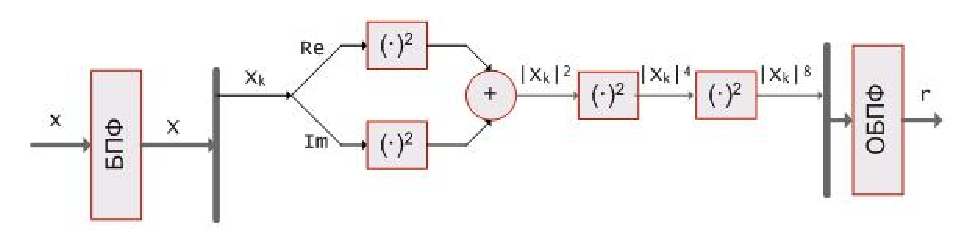
\includegraphics[width=1\linewidth]{akf_fft.eps}}
	\caption{Усовершенствованный итеративный алгоритм получения АКФ}
	\label{pic:akf_pic}
\end{figure}

\newpage
